
\documentclass[british,10pt,a4paper]{article}
\usepackage[british]{babel}
\usepackage[margin=1in, bottom=0.75in, top=0.75in, footskip=0.25in]{geometry}
\usepackage[titletoc]{appendix}
\usepackage{fancyhdr}
\usepackage{mathtools}
\usepackage[numbers]{natbib}
\usepackage{filecontents}
\usepackage{pgfplots, pgfplotstable}
    \pgfplotsset{%
    	% every tick label/.append style={scale=1.5},
        compat=newest,%
        /pgf/number format/use comma,%
        /pgf/number format/1000 sep={\,},%
        /pgf/number format/min exponent for 1000 sep=4}
\usepgfplotslibrary{statistics}
\usepackage{hyperref}
\usepackage{booktabs}
\usepackage{wrapfig}
\usepackage{listings}
\usepackage{color}
\usepackage{graphicx}
\usepackage{siunitx}
\usepackage[parfill]{parskip}
\usepackage{tikz} % To generate the plot from csv
\usepackage{float}

\pgfplotsset{compat=newest} % Allows to place the legend below plot
\usepgfplotslibrary{units} % Allows to enter the units nicely

\graphicspath{ {images/} }

\setcounter{secnumdepth}{2}
\setcounter{tocdepth}{2}
\renewcommand{\arraystretch}{1.2}
\renewcommand\thesection{\arabic{section}}
\renewcommand\thesubsection{\roman{subsection}.}
\renewcommand\thesubsubsection{}
\newcommand*{\Appendixautorefname}{appendix}
\pagestyle{fancy}
\fancyhf{}
\renewcommand{\headrulewidth}{0pt}
\lfoot{Exam no: Y0076159}
\cfoot{\thepage}
\lstset{
  columns=fixed,
  breaklines=true,
  basicstyle=\ttfamily\footnotesize
  }

\usepackage[nottoc]{tocbibind}
\usepackage{csvsimple}

\begin{document}
\title{EVCO Open Assessment}
\author{Exam no: Y0076159}
\date{\today}
\maketitle
\tableofcontents
\clearpage
\listoffigures
\clearpage


\section{Introduction \& Problem Definition}

\begin{minipage}{0.7\textwidth}
The game of Snake was first invented in 1976, as an arcade game named 'Blockade', and later as a computer game named 'Worms' for the TRS-80 microcomputer in 1978 \cite{Goggin2010-ao}; it gained a huge traction on mobile phones following Nokia engineer Taneli Armanto's implementation of the game for the Nokia N6110, released in 2002 \cite{Goggin2010-ao}. The game, in which a single player controls a 'snake' composed of a dot, square or object, is named after the way in which the body of the dot, square or object trails behind the dot controlled by the player. The player can turn the snake's head to change it's direction of travel, whilst the forward movement is uniform relative to time (the player has no control over the speed at which the snake moves). The player aims to win the game by collecting food places on the screen, with every item of food eaten causing the snake's tail to grow. As the player eats more food, the tail grows longer, and it becomes more difficult to navigate the plane without colliding with a surrounding wall, or the player's tail: these form the 2 losing conditions, whilst a player who successfully grows his snake to cover the entire plane has beaten the game.  \newline
Our version of the game is restricted to a 12x12 grid (144 spaces), surrounded by walls, with a single piece of food present on the board at any given time. Furthermore, the snake can go in any one of 4 directions (north, south, west, east), and always advances by 1 square at a time along either the X or Y axis of the board. As the snake is initialised with a body of size 11, the maximal score obtainable is $144-11=133$), at which point food cannot be placed on a tile not occupied by the snake's body. 
\end{minipage}
\begin{minipage}{0.02\textwidth}
\end{minipage}
\begin{minipage}{0.28\textwidth}
	\begin{figure}[H]
	\centering
		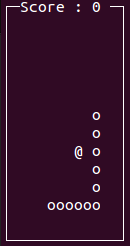
\includegraphics[width=3cm,keepaspectratio]{images/snake.png}
		\caption{A game of snake as simulated in our environment.}
		\label{fig:snake}
	\end{figure}
\end{minipage}
Within the context of this project, we will be aiming to produce an evolutionary algorithm (i.e: an algorithm capable of producing a game-winning A.I. from a set of logical connectives and in-game actions) which can beat the game. That is, we will aim to maximise the number of pieces of food eaten in a run of the game. Key challenges will likely be:
\begin{itemize}
	\item To ensure the snake does not collide into it's own tail or the surrounding walls.
	\item To ensure the snake successfully eats the next piece of food without timing out.
	\item To ensure the algorithm can be run relatively quickly, so it can be evaluated over a large number of runs for statistical analysis.
\end{itemize}

\section{Literature review}
\subsection{Genetic algorithms}
Evolutionary computing is a form of algorithms which seek to find a solution to a problem through a process similar to biological evolution. \cite{Ashlock_undated-vx} The general concept involves initialising a set of candidate solutions, and iteratively updating them to obtain a 'fitter' solution. This is effectively implemented by assessing each candidate using a fitness function, before selecting a a subset of solutions which will be allowed to be bred into child solutions, mutated, and inserted into the next generation's population. This causes the overall fitness of the population to grow over the cycle of evolution, creating a candidate solution which will be closer to the global optimum. Algorithms which implement this evolutionary cycle are known as evolutionary algorithms. The field of evolutionary algorithms (EA) is sub-divided into a series of genetic representations and implementation systems. We will first discuss each of these, highlighting key papers and applications of each to our current situation.\newline

\subsubsection{Genetic algorithm}
A genetic algorithm (GA's) traditionally represent the genotype of a candidate using a binary string, although other representations are possible \cite{Whitley1994-tx}. It is extremely effective at tuning parameters of a model, as demonstrated by \citet{Wloch2004-vo} who used a GA to optimise the parameters of a simulated Formula One car, allowing it to minimise it's lap time. GA's have been implemented for use in the snake game by \citet{Yeh2016-ts}; the algorithm functioned by adjusting the rating functions of 4 operations, each of which decided the snake's next move based on either minimising the number of turns, the free space surrounding the head, or the presence of food near the snake's head. This enabled the snake to evolve a variety of solutions formed of varying frequencies of each function, resulting in a snake capable of beating the game (collecting the maximal number of food possible, where the snake's body fills the entire plane). As the snake's behaviour is not analysed by any means other than it's score in the game, it is difficult to know whether the solution reflected an EA's ability to create novel solutions to the problem. Due to this (and the restrictions on hard-coding solutions to this assessment), an approach using genetic programming was considered, as seen in \autoref{subsec:gp}.

\subsubsection{Genetic programming}
\label{subsec:gp}
Genetic programming (GP) utilises a tree structure to define the genotype of a candidate solution \cite{Cramer_undated-bj}. Nodes in the tree represent certain operators, with leaf nodes representing operands. This allows a decision tree to be evolved, which can rely on conditionally verifying various functions, and applying a move depending on the values of these functions; an example of this is analysed in \autoref{subsec:gp_snake}. Other examples of applications of GPs to games can be found in \citet{Hauptman2005-zg}, who evolved a chess playing agent using a GP. It has also been used in other video games, such as a tower defence game \cite{Leong2013-pu}, space invaders, froggers and missile command \cite{Jia2015-jk}. Within the context of defining a program, GP produce invalid states less frequently than genetic algorithms, as they can be strongly typed (such as in \cite{Jia2015-jk} to ensure that the syntax of the defined operations conforms to an executable standard \cite{Chen2012-ei}. As such, it provides an easily analysable solution to the creation of a snake A.I, as the output of a function is a readily human-readable output. It's additional efficiency in evolving further maximises it's capabilities towards our problem.

\subsection{Grammatical Evolution}
\begin{figure}
\centering
	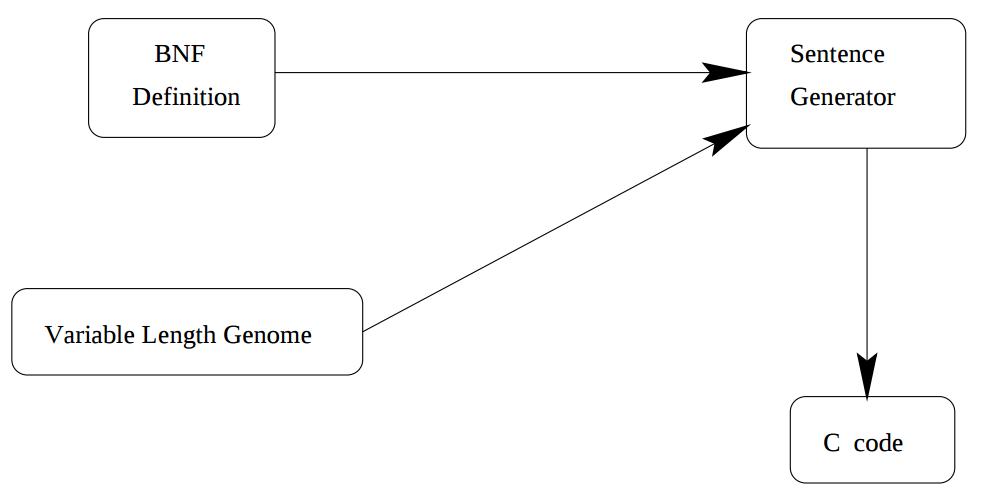
\includegraphics[width=12cm,keepaspectratio]{images/ge.png}
	\caption{The process of grammatical evolution. Source: \cite{ryan:1998:geepal}}
	\label{fig:ge}
\end{figure}
Grammatical evolution (GE) presents the next development in EA's; as with genetic programming, it aims to produce a section of code which can define a function, solving the problem at hand. As detailed by \citet{ryan:1998:geepal}, it aims to avoid the requirements of closure imposed on solutions in genetic programming, which are the main causes of bloating and limitations in crossovers. This is circumvented by the use of a user-specific grammar in Backus-Naur form, restricting the search space to only valid individuals. In contrast to a GP, it splits a genotype and phenotype; that is, the objects operated on by the search algorithm differ from those evaluted by the fitness function. This occurs as the grammar is converted into a program through the use of codons, which index the child element to select for each element in a BNF. This process is illustrated in \autoref{fig:ge}, although within the case of this project our code will be produced in Python 2.7.3. As such, GE's provide an escape from the problems suffered by GP's, without adding any significant complexity: this is reflected by a significant improvement in performance when compared to GP's, as demonstrated by \citet{Michael_ONeill1999-zi}. In this paper, GP's and GE's were implemented to solve the Santa Fe ant trail issue, demonstrating a greatly improved fitness for GE's when evolved over the same number of generations as GP's; this is visible in \autoref{fig:gp_vs_ge}. It is therefore apparent that a GE would be more appropriate than a GP to solve the Snake game, but as it is not natively available in the DEAP \cite{deap}, implementing it would go beyond the scope of this project; therefore, a GP will be used.


\begin{figure}
\centering
	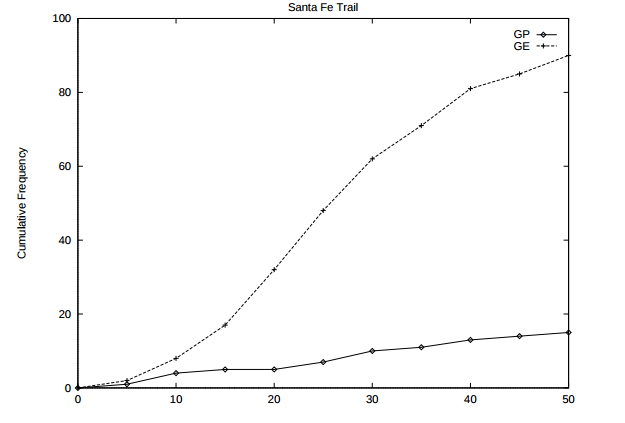
\includegraphics[width=12cm,keepaspectratio]{images/gp_vs_ge.png}
	\caption{GE in comparison to GP, Source: \cite{Michael_ONeill1999-zi}}
	\label{fig:gp_vs_ge}
\end{figure}

\subsection{Neuro-evolution}
Neuro-evolution presents the third viable algorithm for the snake game. In this scheme, a neural network's topology and weights are evolved to develop a network which can sense various parameters from it's environment, and output an optimal action back into the game. This was well demonstrated by \citet{Hausknecht2014-uc}, who evolved a single network capable of beating human high scores in a variety of Atari 2600 games. It has also been used to play simple board games, such as Tic-Tac-Toe \cite{Fogel1993-qp}, or GO \cite{Richards1998-si}. As such neuro-evolution is an extremely potent methodology, and further work in it's implementation for the snake game is worthwhile, but it's unavailability in DEAP restricts it's usage for this project. Furthermore, we could hypothesise that a neuro-evolution approach to a simple problem such as the one at hand (relative to playing 61 different games with the same network) may result in a solution which is difficult to analyse, and potentially excessively large in comparison to a GP/GE approach.

\subsection{Co-evolution}
Finally, the last applicable evolutionary technology considered for this application is co-evolution (differential evolution, gene expression programming and evolution strategies were also considered but found to be no more powerful than a GE or GP algorithm within the context of this problem). Co-evolution allows a second population to be evolved in parallel to the first, such that the fitness of an individual in one's population is evaluated using individuals from the other population. This can be combined with any of the previously discussed techniques by running a pair of the algorithms in tandem; however, as we will later detail, it is possible to develop a solution to the snake game which is independent from the size of the map, or the placement of food. As such, there is no competitive development which could be obtained from evolving a map, and therefore co-evolution would not be beneficial to this experiment.


\subsection{Applications of artificial intelligence to Snake}
Some research has also been undertaken to develop intelligent agents for the snake game: \citet{Bowei_Ma_undated-tl} has described an approach to reinforcement learning using Q-learning and SARSA through neural networks, but do not provide any applicable innovation to a GP-based implementation as they use a simple score-based fitness function and a completely different algorithm.  [TODO expand]

\subsection{Genetic programming for snake}
\label{subsec:gp_snake}
\citet{Ehlis2000-sz} has provided the only comprehensive article specific to the applications of genetic algorithms to Snake. The definitions of the problem diverge from our assessment in a few non-essential ways: snake movements can be inherently defined relative to the snake's current direction (i.e: a turn\_right and turn\_left terminal is defined), and the playing field of the game is a larger rectangle than the 12\*12 field. In all other respects, \citeauthor{Ehlis2000-sz} provides
an overview of a method which functions on the same game as our case. Given this, we will first analyse this approach to the problem, and aim to build an improvement both in terms of computational performance and quality of the solution. \newline

A generic set of terminals allowing the snake to navigate the world is defined: Forward, Left and Right. The latter two allow the snake to make a change of direction relative to it's current heading, whilst the first argument does not affect the heading. The relative movement provided by the two turn operators does allow for a simpler evolution, as implementing an equivalent relative turn using absolute directions requires a significant number of operators, as we will later discuss \autoref{subsec:design_terminals}. \newline

Non terminals can be categorised as either food sensing (ifFoodAhead, ifFoodUp, ifFoodRight) or danger sensing (ifDangerAhead, ifDangerRight, ifDangerLeft, ifDangerTwoAhead). The use of absolute food sensing (ifFoodUp, ifFoodRight) does however require the addition of 4 sensing methods to orient the snake, allowing it to undertake the correct action given the context. This introduces some complexity into the set of operators, potentially limiting the efficiency of the algorithm.\newline

These sets of operators therefore define a generally greedy behaviour: the snake may be progressing towards the food, either at the root of the decision tree or further down once a given situation occurs (such as the 'wall-slitherer' describes in \cite{Ehlis2000-sz}). This evokes a classical approach to the game, similar to what we could expect from the average player\'s strategy. However, given that the last move of a game-winning situation would involve fully covering the map, a greedy approach would need to be very attentive to surrounding dangers to correctly navigate a path to the wall. As such, the difficulty a greedier snake may have in adapting to every potential situation may be the cause for why the algorithm may not produce optimal solutions: an example situation is stated by \citeauthor{Ehlis2000-sz}. This issue forms a basis for the design as later explained. \newline

Some novel features are implemented in this algorithm: the use of multiple evaluations on every snake at every generation cause a larger cost in computational requirements, but do greatly improve the robustness of the solution to food placement and limit the effects of lucky/unlucky food placement on the performance of a snake. Similarly, the fitness function punishes snakes which do not find any pieces of food, thereby promoting snakes which search for the food. The algorithm also relies on priming the population of individuals, by selecting well-performing pre-produced solutions in the initial breeding pool.

Additional details of the algorithm are however lacking: a large population of 10000 individuals is evolved for 500 generations; the large population is potentially a counterweight to the lack of mutation, as unique genomes are created at the start of the evolution rather than during it; this most likely results in an equivalent effect. with a maximum tree size of 150 nodes to limit bloating. Crossover probability is stated as .10 for leaves, 0.80 for nodes, with a mutation probability of 0, in addition to the use of primed populations from previously unsuccessful runs. Additional details concerning which mutation or crossover functions were used are omitted, and reasonable assumptions of these are discussed in \autoref{subsec:impl} to evaluate the method. The algorithm did however account for the randomisation of food placement, mitigating it by evaluating each individual over multiple runs per generation; this was also considered in our algorithm, as we will later discuss.\newline

The proposed solution results in the creation of a game-winning decision tree (which scores the maximal 211 points). This algorithm was re-implemented to establish a benchmark for our research, revealing a significant requirement in computational time, as discussed in \autoref{subsec:impl}.

\subsection{Implementation, assumptions and results}
\label{subsec:impl}
In order to obtain benchmark fitness values, tree sizes and computational times against which to evaluate our new algorithms, the algorithm developed by \citeauthor{Ehlis2000-sz} was implemented using the Python DEAP \cite{deap} package; the code for this can be found in \autoref{app:approach1}. \newline

The algorithm was ran 30 times in order to obtain a reliable statistic of it's performance when provided with the population size and computational resources proposed by \citeauthor{Ehlis2000-sz}.
Given that approximately 30 hours of computational time were required to evaluate this, a subsequent evaluation (using a population of 1000, and 150 generations) was run to obtain results against which we can compare our new algorithms quickly. Some assumptions regarding the type of mutation were made: uniform tree insertion was first considered, but as the crossover was set to probability 0, this would be unable to grow the tree. Therefore, a uniform mutation which inserts a subtree of depth 1-3 was utilised. Crossover was set with a probability of 0.0 as per \citeauthor{Ehlis2000-sz}'s design. Finally, we assumed that the fitness tournament was used to drive the population's average fitness upwards: this was implemented with a size of 2, and that a standard evolution algorithm was used (DEAP's eaSimple).\newline

\begin{figure}
\centering
\resizebox {!} {7cm} {
	\begin{tikzpicture}[font=\LARGE]
	    \begin{axis}[xlabel=Food Eaten, ylabel=Count, ybar,xtick=,width=\textwidth]

	    \addplot+[
	    	hist={
	    		data=x,
	    		bins=14,
	    		data min = 0,
	    		data max = 134
	    	}]
	            file [y index=0]  {data/approach1.csv};
	\end{axis}
	\end{tikzpicture}
}
\caption{Histogram of best individuals from \citeauthor{Ehlis2000-sz}'s algorithm, 500 generations, 10,000 population}
\label{fig:approach1}
\end{figure}

As seen in \autoref{fig:approach1}, the algorithm produced 8 optimal solutions (a maximal score of 133), and an average best individual of 92.06 pieces of food eaten (std: 45.64). One should note that the algorithm only has a 33.3\% success rate in producing game-beating snakes; this is certainly related to the shortening of the algorithm by 350 generations, and the algorithm may therefore be more successful than the results above. \newline

When limited to a practical computational time (150 gens at 1000 population), the algorithm performs equivalently well, with an average of 97.97 pieces of food eaten, and a smaller standard deviation of 29.79 over 30 runs. This highlights the volatility of the algorithm, as well as the need for a large population or a larger number of generation to obtain an optimal value. Nevertheless, we can establish a benchmark against which we can compare future algorithms, keeping in mind the scale of resources provided to the algorithms is limited given available computing power. This can most easily be described as an average best score of 97.97  (std: 29.79), given 150 generations with a population of 10 00, with an average tree size of 362.8 nodes. \newline

\section{Testing \& Design methodology}
In order to evaluate the effects of operators or fitness functions, each candidate fitness function will be evaluated 30 times, with a consistent configuration: a population of 1000 individuals evolved over 150 generations. We will aim to create an algorithm which requires less computational power, and produces optimal results more consistently with a smaller population and tree size. Fitness functions will be evaluated using the same algorithm (eaSimple), although a later comparison of algorithms will be run. Finally the optimal mutation and crossover probabilities will be found by iterating combinations of them with the most promising algorithm. As the benchmark algorithm discussed in \autoref{subsec:impl} does not produce normally distributed data (as visually verifiable using the graph), a Mann-Whitney U-test will be used to compare the score of subsequent algorithms, as it does not rely on the assumption of normal distributions.

\section{Design \& implementation}
\subsection{Evolutionary algorithm}
A genetic programming algorithm was used, as it provided the most flexibility available from the DEAP package in terms of the solution space explored as it utilised a large number of operators, each with a small individual impact over the snake's movement, in comparison to an implementation which utilised a genetic algorithm such as \citet{Yeh2016-ts}.

\subsection{Strategy}
As \citet{Ehlis2000-sz} has already demonstrated a game-beating A.I, it was decided to focus on 3 aspects which we could compare to this algorithm:
\begin{itemize}
	\item Equalling or beating the reliability of the algorithm
	\item Reducing the computational time
	\item Reducing the size of the average game-beating solution
\end{itemize}
Building on the work by \citeauthor{Ehlis2000-sz}, we will aim to adapt his design to our requirements whilst improving it. \newline

As noted by \citet{Christopher_Lockhart2010-em} in his publication about difference learning in Snake, "the greedy behaviour of [a learning agent] may be the cause of the agent's lack of high scores. Whilst this is disproven by the success rate of \citeauthor{Ehlis2000-sz}\'s algorithm, we could argue that given a sufficiently large population, a set of operators can produce any solution which could also be produced by a subset of those operators. We attempted to demonstrate this in \autoref{fig:operator_prob}, where we compiled statistics from the best individuals of optimal (game-winning with a score of 133) and non-optimal solutions, across 30 runs with a population of 10 000 and 150 generations. As we can see, there is no noticeable difference between the frequency of operators, thereby demonstrating that not all optimal solutions are greedy, as this would be reflected by a lower percentage of food sensing functions (redundancies in the graphs (such as repeated operators or unrecheable branches) and noise in the data obtained may also have obscured any visible pattern). Nevertheless, we will hypothesise that developing a non-greedy snake may have the following benefits.

\begin{figure}
\centering
	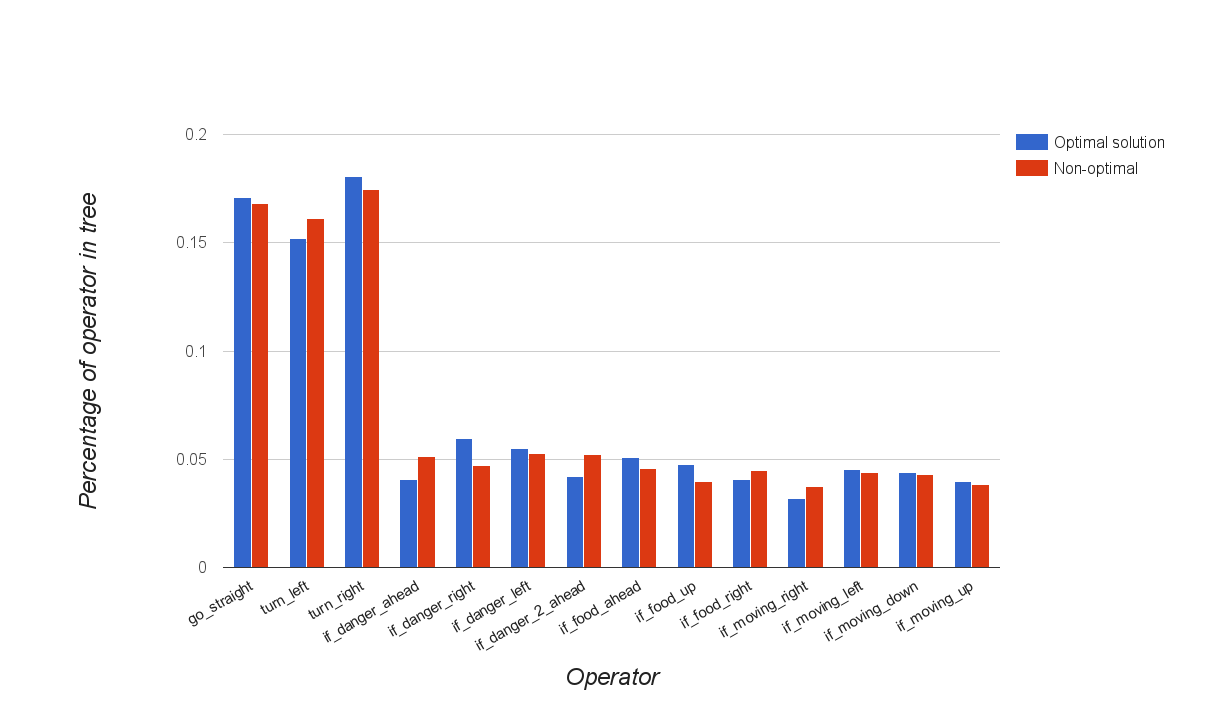
\includegraphics[width=\textwidth,keepaspectratio]{images/operator_prob.png}
	\caption{Difference in statistics of operators between optimal and non-optimal solutions}
	\label{fig:operator_prob}
\end{figure}

\begin{itemize}
	\item A greedy snake which alters it's movement based on the positioning of food is likely to require additional sensing to avoid going causing game-ending situations, such as entering a dead-end to get closer to a piece of food. This would require the handling of many edge cases, which will cause the need for a large solution, which is therefore difficult to evolve. A non-greedy snake, which would aim to find a hamiltonian cycle through the map such that it's tail will never be in it's direct path until it has reached maximal size, could require a significantly smaller function to define it; this should make it easier to evolve, and therefore increase the reliability and speed of the algorithm.
	\item As a non-greedy snake would not sense food, it's fitness is unlikely to be greatly affected by the positioning of food. Therefore, it may not be necessary to evaluate each individual multiple times, which was done to improve the robustness of the solution in \cite{Ehlis2000-sz}.
\end{itemize}
Due to this, it was decided to aim for a non-greedy solution which would not sense for food, but would rather aim to explore the map in a maximal way; this would adequately resolve the prescribed goal of beating the game by obtaining a maximal score, even though it may not be achieved in a minimalistic way.



\subsection{Terminal and Non-terminal set}
\label{subsec:design_terminals}
The most significant difference of environment between our project and previous work involves the added complexity of using only absolute turning: as such, instead of a simple turn\_left and turn\_right function, we implement changeDirectionUp, changeDirectionRight, changeDirectionDown, changeDirectionLeft; these allow the snake's head to progress towards one of 4 directions at the next move. As these directions are difficult to use without any knowledge of the current heading (e.g: turning down when going north would cause the snake to reverse into it's own body), an additional 4 senses are used: if\_moving\_up, if\_moving\_down, if\_moving\_left, and if\_moving\_right. \newline

As we will aim for a non-greedy solution, food sensing is not implemented in the new algorithm. We will aim to produce a hamiltonian cycle (where every space of the bordered plane is visited only once before returning to the original), as this will avoid having to take the snake's tail into consideration. Therefore, we will implement 4 wall-sensing functions: sense\_wall\_ahead, sense\_wall\_left, sense\_wall\_right and sense\_wall\_2\_away. The first 3 of these are relative to the snake's orientation, and allow the snake to navigate against a wall, whereas the the 4th sense allows the snake to avoid completely traversing the map along either the X or Y axis, thereby permitting it to avoid cutting itself off from part of the map which will be made available as it continues to move. \newline
\begin{table}[]
\centering
\caption{Operators}
\label{tab:operators}
\begin{tabular}{|l|l|}
\hline
\textbf{Terminal} & \textbf{Non-terminal} \\ \hline
go\_straight      & if\_wall\_2\_away     \\ \hline
go\_up            & if\_wall\_left        \\ \hline
go\_down          & if\_wall\_right       \\ \hline
go\_right         & if\_wall\_ahead       \\ \hline
go\_left          & if\_moving\_up        \\ \hline
                  & if\_moving\_down      \\ \hline
                  & if\_moving\_left      \\ \hline
                  & if\_moving\_right     \\ \hline
\end{tabular}
\end{table}
We have therefore created a small 13 operator set which can be used to produce a non-greedy snake.
\subsection{Fitness function}
Keeping in line with the aim of a greedy snake, our fitness function does not include the snake's score in the game; this is due to the fact that snakes cannot sense food, and therefore their score will be directly correlated with the distance travelled by the snake (and therefore it's distance travelled, as it moves at a constant speed). In addition, as the snake's score can greatly be influenced by the random placement of food in the starting few generations, removing the scoring of food reduces the skewing of a snake's fitness due to lucky food placing. This further reduces the need to evaluate each snake multiple times, as the snake only reacts relative to constant objects in the plane (4 walls). Finally, to ensure the hamiltonian cycle covers every square of the map, we introduce the notion of a cover to the fitness function, which is equal to the proportion of the map visited by the snake during the run. This ensures that snakes develop a maximal coverage of the map, so that it can grow to a maximal size. \newline
We can therefore define the fitness function as \(fitness= (\% \ of\ map\ covered) + (steps/100)\). \newline
In addition to this, we also implemented a penalty for snakes which enter a non-maximal loop: this is implemented by checking if the snake has timed out (i.e has travelled 196 steps without collecting food). This removes problematic solutions from the early stages of evolution, as these individuals would otherwise score highly due to their long survival; instead, they will now be assigned a fitness of -10, thereby greatly reducing their likelihood of selection, and therefore their effect on the population's genotype.

\subsection{Creation of individuals}
\subsection{Selection, Mutation \& Crossover}
As details of the selection algorithm in \cite{Ehlis2000-sz} are sparse, we decided to utilise a double tournament, to ensure that the size of the solutions was minimised given an equal fitness. As such, DEAP's 

In contrast to \citeauthor{Ehlis2000-sz}\'s algorithm, which relied on the insertion of trees in the place of individual nodes to grow a solution beyond it's initial size (as crossover probability was set to 0), our genetic algorithm utilises crossover throughout it's evolution. Therefore, it was possible to rely on crossover to grow a tree's size, whilst DEAP's mutNodeReplacement operator, which replaces a primitive from an individual by any other primitive which has the same number of arguments, was used to mutate individuals. This allows nodes within the tree to be replaced with more appropriate nodes, thereby improving their fitness. \newline

The basic one point crossover operator was used, without bias for leaf nodes. \newline
http://ir.library.louisville.edu/cgi/viewcontent.cgi?article=1847&context=etd
\subsection{Parameter selection}
Mutation/Crossover probability
\TODO pull rates from teaching0

\subsection{GP Algorithm selection}
eaSimple vs eaMewCommaLambda
\subsection{Bloat control}
Bloat control was implemented using decorators on the crossover and mutation functions
\TODO experiment with parsimony sizes once crossover/mutation complete

\section{Code optimisation}
\begin{itemize}
	\item Reduced timeout limit to board size
	\item Used Deque to speed up pre-pending and popping from snake body
	\item Single evaluation required 
\end{itemize}
\section{Results and analysis}
\section{Conclusion}
Optimal seed: \lstinline{python approach4.py --seed 0.507299291138} for 50 gens
\TODO verify seeding is correct
\subsection{Further work}
\begin{itemize}
	\item Taking a population of optimal solutions, giving them more operators and evolving a more efficient A.I. which wins the game in the smallest time possible
	\item Testing the ability to improve the reliability of the algorithm using larger populations, 
\end{itemize}

\clearpage

\bibliographystyle{IEEEtranSN}
\bibliography{references}
\clearpage
\begin{appendices}

	\section{Benchmark algorithm}\label{app:approach1}
	Based on the design document by \citet{Ehlis2000-sz}. \newline
	\lstinputlisting[language=Python]{../GP/approach1.py}
  	\clearpage	

	\section{New algorithm}\label{app:approach4}
	Based on the design document by \citet{Ehlis2000-sz}. \newline
	\lstinputlisting[language=Python]{../GP/approach4.py}
  	\clearpage	

\end{appendices}
\clearpage
\end{document}
